\documentclass[letterpaper, 12pt]{article}

%%%%%%%%%%%%%%%%%%%%%%%%%%%%%
% DEFINITIONS
% Change those informations
% If you need umlauts you have to escape them, e.g. for an ü you have to write \"u
\gdef\mytitle{Protokoll}
\gdef\mythema{Continuous Integration}

\gdef\mysubject{SEW}
\gdef\mycourse{5BHIT 2015/16}
\gdef\myauthor{Michael Weinberger}

\gdef\myversion{1.0}
\gdef\mybegin{9. Februar 2016}
\gdef\myfinish{16. Februar 2016}

\gdef\mygrade{Note:}
\gdef\myteacher{Betreuer: Dolezal/Vittori}
%
%%%%%%%%%%%%%%%%%%%%%%%%%%%%%

\input special/preamble.tex

\let\tempsection\section
\renewcommand\section[1]{\vspace{-0.3cm}\tempsection{#1}\vspace{-0.3cm}}
\WithSuffix\newcommand\section*[1]{\tempsection*{#1}}

\let\tempsubsection\subsection
\renewcommand\subsection[1]{\vspace{0cm}\tempsubsection{#1}\vspace{0cm}}

\let\tempsubsubsection\subsubsection
\renewcommand\subsubsection[1]{\vspace{0cm}\tempsubsubsection{#1}\vspace{0cm}}

\linespread{0.94}

\lhead{\mysubject}
\chead{}
\rhead{\bfseries\mythema}
\lfoot{\mycourse}
\cfoot{\thepage}
% Creative Commons license BY
% http://creativecommons.org/licenses/?lang=de
\rfoot{\ccby\hspace{2mm}\myauthor}
\renewcommand{\headrulewidth}{0.4pt}
\renewcommand{\footrulewidth}{0.4pt}

\begin{document}
\parindent 0pt
\parskip 6pt

\pagenumbering{Roman} 
%!TEX root=../laborprotokoll.tex

\begin{titlepage}

	\begin{figure}[!h]
		\begin{flushright}
			
\includegraphics[width=0.3\linewidth]{images/jdIT_tgm.png}
		\end{flushright}
	\end{figure}

	\vspace{2.5cm} 

	{\begin{center} \bfseries\huge
			\rule{17.5cm}{0.1mm}  
			\\[5mm]
			\mytitle\\[5mm]
			\mythema\\
			\rule{17.5cm}{0.1mm}  
	\end{center}}

	{\begin{flushright} \bfseries\Large
			\vspace{2cm}
			\mysubject\\
			\mycourse\\[10mm]
			\myauthor\\[10mm]
	\end{flushright}}

	{\begin{table}[!h] \bfseries\normalsize
		\begin{tabularx}{\textwidth}{lXr @{\hspace{0mm}}}
			&& Version \myversion\\
			\mygrade && Begonnen am \mybegin\\
			\myteacher && Beendet am \myfinish\\
		\end{tabularx}
	\end{table}}

\end{titlepage}


\clearpage
\thispagestyle{empty}
\tableofcontents

\newpage
\pagenumbering{arabic}
\pagestyle{fancy}

%\vspace{-0.5cm}
\section{Einführung}
\textit{"Continuous Integration is a software development practice where members of a team integrate their work frequently, usually each person integrates at least daily - leading to multiple integrations per day. Each integration is verified by an automated build (including test) to detect integration errors as quickly as possible. Many teams find that this approach leads to significantly reduced integration problems and allows a team to develop cohesive software more rapidly. This article is a quick overview of Continuous Integration summarizing the technique and its current usage." M.Fowler} \\ \\

Schreibe fünf Testfälle für dein CSV-Projekt und lass diese mithilfe von Jenkins automatisch bei jedem Build testen!

\begin{itemize}
	\item Installiere auf deinem Rechner bzw. einer virtuellen Instanz das Continuous Integration System Jenkins
	\item Installiere die notwendigen Plugins für Jenkins (Git Plugin, Violations, Cobertura)
	\item Installiere Nose und Pylint (mithilfe von pip)
	\item Integriere dein CSV-Projekt in Jenkins, indem du es mit Git verbindest
	\item Schreibe fünf Unit Tests für dein CSV-Projekt
	\item Konfiguriere Jenkins so, dass deine Unit Tests automatisch bei jedem Build durchgeführt werden inkl. Berichte über erfolgreiche/fehlgeschlagene Tests und Coverage
	\item Protokolliere deine Vorgehensweise (inkl. Zeitaufwand, Konfiguration, Probleme) und die Ergebnisse (viele Screenshots!)
\end{itemize}

Viel Spaß! :)
\newpage

\section{Durchführung}

\subsection{Jenkins installieren}
Ich habe mich entschieden Jenkins in einer virtuellen Instanz zu installieren. Verwendet wurde Ubuntu 15.10 unter VMware Workstation 12. Folgende Befehle waren notwendig: \\

\begin{lstlisting}[frame=single,language=bash, caption=Jenkins in Ubuntu installieren \cite{jenkins}]
wget -q -O - https://jenkins-ci.org/debian/jenkins-ci.org.key | sudo apt-key add -
sudo sh -c 'echo deb http://pkg.jenkins-ci.org/debian binary/ > /etc/apt/sources.list.d/jenkins.list'
sudo apt-get update
sudo apt-get install jenkins
\end{lstlisting}

Sollte der Port 8080 bereits belegt sein und /etc/init.d/jenkins fehlschlägt, muss in /etc/default/jenkins der Wert bspw. auf 'HTTP\_PORT=8081' gesetzt werden.

\subsection{Installieren der notwendigen Plugins}
Im Menüpunkt 'Jenkins verwalten' findet sich der Punkt 'Plugins verwalten'. Im Reiter 'Verfügbar' lassen sich die drei benötigten Plugins \texttt{Git Plugin, Violations \& Cobertura} auswählen und installieren, Jenkins wird per Klick auf die Checkbox neu gestartet, damit die Erweiterungen auch ausgeführt werden. \\
Das Git Plugin integriert, wie der Name sagt, die Git-Unterstützung in Jenkins, zusätzlich habe ich das Github Authentication Plugin installiert, um eine Authentifizierung per Github OAuth zu gewährleisten. Violations überprüft den Code auf Verstöße gegen Coding-Richtlinien, und Cobertura stellt Coverage-Reports bereit. 

\subsection{Installieren von Nose und Pylint}

\begin{lstlisting}[frame=single,language=bash, caption=Nose und Pylint mit pip installieren]
sudo pip install nose
sudo pip install pylint
\end{lstlisting}

\texttt{Nose} kümmert sich um Unittests, und \texttt{Pylint} überprüft den Code auf Fehler, und versucht einen bestimmten Codestandard zu erreichen. \\

\newpage

\subsection{Integriere dein CSV-Projekt in Jenkins, indem du es mit Git verbindest}

Die nächsten Schritte habe ich aus dem Tutorial übernommen. \cite{steveblog} \\ \\
Unterpunkte: 
\begin{itemize}
	\item Our first job
	\item 1 - Where to get the source
	\item 2 - When to run the job
	\item 3 - What to run \\\\
	Wichtig! Hier die Shell je nach System selbst anpassen!
	\item 4 - Interpret the results \\\\
	Auch hier einige wichtige Schritte, dieses Mal um die Plugins richtig zu verwenden.
	\item Run the job
\end{itemize}

\subsection{Konfiguriere Jenkins so, dass deine Unit Tests automatisch bei jedem Build durchgeführt werden inkl. Berichte über erfolgreiche / fehlgeschlagene Tests und Coverage}

Ein erster Build wird fertiggestellt mit folgendem Output:

\begin{lstlisting}[frame=single,language=bash, caption=Build \#1]
Started by an SCM change
Building in workspace /var/lib/jenkins/jobs/csv/workspace
> git rev-parse --is-inside-work-tree # timeout=10
Fetching changes from the remote Git repository
> git config remote.origin.url https://github.com/mweinberger-tgm/Continuous-Integration.git #
timeout=10
Fetching upstream changes from https://github.com/mweinberger-tgm/Continuous-Integration.git
> git --version # timeout=10
> git -c core.askpass=true fetch --tags --progress https://github.com/mweinberger-tgm/Continuous-Integration.git
+refs/heads/*:refs/remotes/origin/*
> git rev-parse refs/remotes/origin/master^{commit} # timeout=10
> git rev-parse refs/remotes/origin/origin/master^{commit} # timeout=10
Checking out Revision 8c6b0b6d136c67dbdda6e213fe310bfde36b7321
(refs/remotes/origin/master)
> git config core.sparsecheckout # timeout=10
> git checkout -f 8c6b0b6sdfg235sfg324da6e213fe310bfde36b7321
> git rev-list 01c4c4cfef6607d5vfbwedsdfdf235a5507d901e9873 # timeout=10
[workspace] $ /bin/sh -xe /tmp/hudson6843542523459213337267.sh
----------------------------------------------------------------------
Ran 5 tests in 0.040s

...






Mit Shell:

PYTHONPATH=''
Nosetests-3.4 --with-xunit --all-modules --traverse-namespace --with-coverage --cover-package=project1 --cover-inclusive
python -m coverage xml
pylint -f parseable -d I0011,R0801 CSVReader.py | tee pylint.out

\end{lstlisting}

Daraufhin war das gewünschte Ergebnis sichtbar. Link zum Repo \cite{repo}

\begin{figure}[!h]
	\begin{center}
		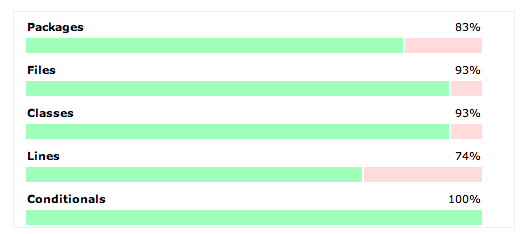
\includegraphics[width=1\linewidth]{images/coverage}
		\caption{Beispiel Code Coverage}
		\label{Beispiel Code Coverage}
	\end{center}
\end{figure}

\clearpage

\bibliographystyle{unsrt}
\bibliography{Continuous-Integration_Weinb_5BHIT}
\lstlistoflistings
\listoffigures

\end{document}
